
% This LaTeX was auto-generated from an M-file by MATLAB.
% To make changes, update the M-file and republish this document.

\documentclass{article}
\usepackage{graphicx}
\usepackage{color}
\usepackage{mcode}
\usepackage{amsmath}
\usepackage{amsfonts}

\sloppy
\definecolor{lightgray}{gray}{0.5}
\setlength{\parindent}{0pt}

\begin{document}

    
    
\section*{DOCUMENT TITLE}

\begin{par}
INTRODUCTORY TEXT
\end{par} \vspace{1em}

\subsection*{Contents}

\begin{itemize}
\setlength{\itemsep}{-1ex}
   \item Clear complete workspace
   \item Read data files
   \item 3D
   \item Set some neccessary parameters
   \item 3D
   \item Compute FFT
   \item Compute correlations
   \item Show graphs
   \item compute length scales
   \item compute 1D spectrum
   \item compute spectrum
   \item compute k vector
   \item compute 1D spectrum
\end{itemize}


\subsection*{Clear complete workspace}

\begin{par}
Its always a good idea to clear the complete workspace and the command window also closing all figures might be helpful. You may also use the header defin some neccessary flags distinguishing bewteen different data sets.
\end{par} \vspace{1em}
\begin{verbatim}
close all
clear all
clc

flag='2D';
datadir='data';
\end{verbatim}


\subsection*{Read data files}

\begin{par}
Read in the data files and measure the time for reading. The output of the tic/toc block is in seconds. What you should get from the tic/toc block is that most of the time is spend during data I/O. The actual computation needs only ??? of the time of the I/O operations.
\end{par} \vspace{1em}


\subsection*{3D}

\begin{verbatim}
if (strcmp('3D',flag))
    tic; % enable timer
    uvel=importdata([datadir,'/',flag,'/uvel']);
    vvel=importdata([datadir,'/',flag,'/vvel']);
    wvel=importdata([datadir,'/',flag,'/wvel']);
    time_reading = toc; % end timer
end
%%% 2D
if (strcmp('2D',flag))
    tic;
    uvel=importdata([datadir,'/',flag,'/uvel']);
    vvel=importdata([datadir,'/',flag,'/vvel']);
    time_reading = toc;
end
\end{verbatim}


\subsection*{Set some neccessary parameters}

\begin{par}
For further computations it is important to define some parmeters of the DNS simulation such as domain size, grid spacing, and the number of grid points.
\end{par} \vspace{1em}


\subsection*{3D}

\begin{verbatim}
if (strcmp('3D',flag))
    dim=256; % number of points in one dimension
    Lx=5e-3; % domain size
    Ly=Lx;
    Lz=Lx;
    dx=Lx/dim; % grid spacing
    dy=dx;
    dz=dx;
    nu=1.7e-5; % viscosity
    u=reshape(uvel,dim,dim,dim); % reshape arrays to have them in 3D
    v=reshape(vvel,dim,dim,dim);
    w=reshape(wvel,dim,dim,dim);
end
%%% 2D
if (strcmp('2D',flag))
    dim=1024; % number of points in one dimension
    Lx=1E-2;  % domain size
    Ly=Lx;
    dx=Lx/dim; % grid spacing
    dy=dx;
    u=reshape(uvel,dim,dim); % reshape arrays to have them in 2D
    v=reshape(vvel,dim,dim);
end
\end{verbatim}


\subsection*{Compute FFT}

\begin{par}
This is the most important part of the script. Since the performance of an actual DFT is rather bad the preferred choice is a FFT. The FFT approach is fastest if the data set to be transformed has a size that is a multiple of two. Thats why the function \textbf{nextpow2} is used to get the next powert of two approximating the dimension \textit{dim} of the data set. As a consequence the data set is zero padded or truncated. \textit{Since the output of an FFT operation is symmetric we only need to save half the transform}.
\end{par} \vspace{1em}
\begin{par}

  \begin{equation}
     \Phi_{ij}(\kappa)=\frac{1}{(2\,\pi)^3}\iiint^{\infty}_{-\infty}
                          R_{ij}(\mathbf{r})\,\mathrm{e}^{-i\mathrm{\kappa}r}
                          \,\mathrm{d}\mathbf{r}
  \end{equation}
After the transformation of all velocity components we have to compute
the velocity correlation tensor $\Phi$ . From theory we know
  \begin{equation}
  (u_i*u_j)=\int_{-\infty}^{\infty}u_i^{*}(\mathbf{x})\,
                  u_j(\mathbf{x}+\mathbf{r})\,\mathrm{d}\mathbf{r}.
  \end{equation}
Since all our data sets are transformed (and we are in the Fourier space)
the last expression can be simply computed by multiplying
  \begin{equation}
      \mathfrak{F}\left\{u_i*u_j\right\} = \alpha\cdot
          \left\{\mathfrak{F}\left\{u_i\right\}\right\}^{*}\cdot
                 \mathfrak{F}\left\{u_j\right\},
  \end{equation}
where $\alpha$ is normalization factor.

\end{par} \vspace{1em}
\begin{verbatim}
if (strcmp('3D',flag))
    tic; % start timer
    NFFT = 2.^nextpow2(size(u)); % next power of 2 fitting the length of u
    u_fft=fftn(u,NFFT); % transform
    %
    NFFT = 2.^nextpow2(size(v));
    v_fft=fftn(v,NFFT);
    %
    NFFT = 2.^nextpow2(size(w));
    w_fft=fftn(w,NFFT);
    time_fft=toc; % get final time for all transformations

    phi_x=u_fft.*conj(u_fft)/dim^6;
    phi_y=v_fft.*conj(v_fft)/dim^6;
    phi_z=w_fft.*conj(w_fft)/dim^6;
end
if (strcmp('2D',flag))
    NFFT = 2.^nextpow2(size(u));
    u_fft=fft2(u,NFFT(1),NFFT(2))./(2*pi)^2; %2pi comes from the definition of FFT
%     u_fft = u_fft(1:NFFT(1)/2+1,1:NFFT(2)/2+1);
    NFFT = 2.^nextpow2(size(v));
    v_fft=fft2(v,NFFT(1),NFFT(2))./(2*pi)^2;
%     v_fft = v_fft(1:NFFT(1)/2+1,1:NFFT(2)/2+1);

    phi_x=u_fft.*conj(u_fft)/size(u,1).^2/size(u,2).^2;
    phi_y=v_fft.*conj(v_fft)/size(v,1).^2/size(v,2).^2;
end
\end{verbatim}


\subsection*{Compute correlations}

\begin{par}
Computing a correlation can be a tedious work (requireing tremendous effort) especially if you have large data sets. From theory it is well known that the multiplication of the transform of a data set and ist complex conjugate give a accurate representation of the correlation function. Using the FFT approach this gives an enormeous speed advantage.
\end{par} \vspace{1em}
\begin{verbatim}
if (strcmp('3D',flag))
    R11=ifftn(u_fft.*conj(u_fft))/dim^3/std2(u)^2;
    R22=ifftn(u_fft.*conj(u_fft))/dim^3/std2(v)^2;
    R33=ifftn(u_fft.*conj(u_fft))/dim^3/std2(w)^2;
    R11=R11(1:round(size(R11,1)/2),1,1);
    R22=R22(1:round(size(R22,1)/2),1,1);
    R33=R33(1:round(size(R33,1)/2),1,1);
    r = linspace(0,Lx/2,dim/2)/(Lx/2);
else
    NFFT = 2.^nextpow2(size(u_fft));
    R1 = ifft2(u_fft.*conj(u_fft),NFFT(1),NFFT(2))...
                ./NFFT(1)./NFFT(2)./std2(u)^2 ...
                .*(2*pi)^4; % scaling due to division by 2*pi
    %
    NFFT = 2.^nextpow2(size(v_fft));
    R2 = ifft2(v_fft.*conj(v_fft),NFFT(1),NFFT(2))...
                ./NFFT(1)./NFFT(2)./std2(v)^2 ...
                .*(2*pi)^4; % scaling due to division by 2*pi
%     R11= ifftn(fftn(u).*conj(fftn(u))/dim^2/std2(u)^2);
%     R22=ifftn(fftn(v).*conj(fftn(v))/dim^2/std2(v)^2);
    R11 = (R1(1:round(size(R1,1)/2),1) + ...
           R2(1,1:round(size(R2,1)/2))')/2;
    R22 = (R2(1:round(size(R2,1)/2),1) + ...
           R1(1,1:round(size(R1,1)/2))')/2;

%     R11 = (R11 + R2(1,1:round(size(R2,1)/2))')/2;

%     r = linspace(0,Lx/2,dim/2)/(Lx/2);
%     test = R11 + r'/2.*gradient(R11,max(diff(r)));
%     plot(r,R11,r,R22,r,test)
%     legend('R11','R22','Equation');
%     h=line([0 1],[0 0],'Color',[0 0 0],'LineWidth',1.0);
end
\end{verbatim}


\subsection*{Show graphs}

\begin{verbatim}
pcolor(fftshift(R1));shading interp;title('R11');
figure
pcolor(fftshift(R2));shading interp;title('R22');
\end{verbatim}

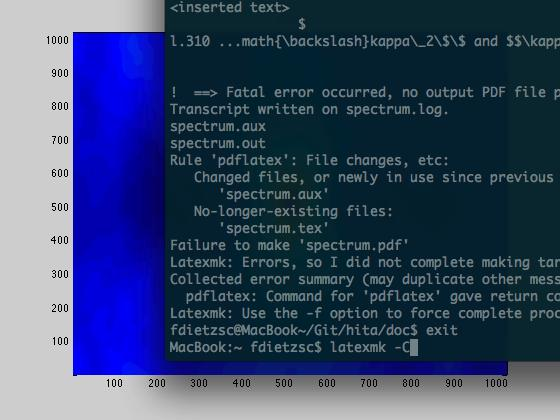
\includegraphics [width=4in]{spectrum_01.jpg}

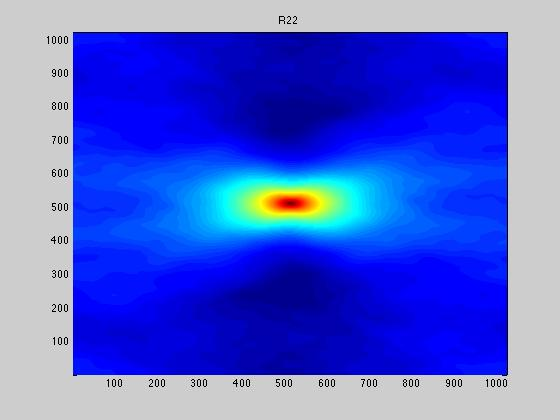
\includegraphics [width=4in]{spectrum_02.jpg}


\subsection*{compute length scales}

\begin{verbatim}
L11=trapz(r,R11);
L22=trapz(r,R22);
hold on
rectangle('Position',[0,0,L11,1],'LineWidth',2,'LineStyle','--')
\end{verbatim}

        \color{lightgray} \begin{verbatim}Undefined function or variable 'r'.

Error in spectrum (line 171)
L11=trapz(r,R11);
\end{verbatim} \color{black}
    

\subsection*{compute 1D spectrum}

\begin{verbatim}
L=length(R1);
NFFT=2^nextpow2(L);
spec_1D=fft(R1(:,1),NFFT)/L.*2/pi;

f = linspace(0,1,NFFT)*2*pi/dx;

slope=1.5*664092^(2/3)*(f.^(-5/3));
% loglog(f,2*abs(spec_(1:NFFT/2+1)));
% hold on
% loglog(f,slope);
\end{verbatim}


\subsection*{compute spectrum}

\begin{par}
spec = zeros(round(dim*dim*dim/8),1);
\end{par} \vspace{1em}
\begin{verbatim}
if (strcmp('3D',flag))
%     phi = u_fft;
%     phi(:,:,:)=0.0;
%     for k=1:dim
%         for j=1:dim
%             for i=1:dim
    %             kappa = sqrt(i*i+j*j+k*k);
    %             kappa_pos=int16(kappa);
    %             if (kappa_pos <= size(spec,1))
    %                 spec(kappa_pos) = spec(kappa_pos)+kappa*kappa*(...
    %                 + real(u_fft(i,j,k))*real(u_fft(i,j,k))+imag(u_fft(i,j,k))*imag(u_fft(i,j,k)) ...
    %                 + real(v_fft(i,j,k))*real(v_fft(i,j,k))+imag(v_fft(i,j,k))*imag(v_fft(i,j,k)) ...
    %                 + real(w_fft(i,j,k))*real(w_fft(i,j,k))+imag(w_fft(i,j,k))*imag(w_fft(i,j,k)));

    %             end
    %             spec(kappa_pos) = spec(kappa_pos) + kappa*kappa*0.5*(phi_x(i,j,k).^+phi_y(i,j,k).^2+phi_z(i,j,k).^2);
                  phi = 0.5*(phi_x+phi_y+phi_z);
                  phi = phi(1:round(size(phi_x,1)/2),...
                            1:round(size(phi_y,1)/2),...
                            1:round(size(phi_z,1)/2));
%             end
%         end
%     end
else
%     phi = u_fft;
%     phi(:,:)=0.0;
%     for j=1:dim
%         for i=1:dim
%             phi(i,j) = phi(i,j) +(phi_x(i,j)+phi_y(i,j));
%         end
%     end
    phi = 0.5*phi_x+phi_y;
    phi = phi(1:round(size(phi_x,1)/2),...
              1:round(size(phi_y,1)/2));
%     phi = phi(1:round(size(phi,1)));
end
\end{verbatim}


\subsection*{compute k vector}

\begin{verbatim}
if (strcmp('3D',flag))
    maxdim = sqrt(dim^2*(2*pi/Lx)^2+dim^2*(2*pi/Ly)^2+dim^2*(2*pi/Lz)^2);
    E=zeros(uint64(sqrt(3*dim^2)),1);
    kk=zeros(uint64(sqrt(3*dim^2)),1);
    dim = size(phi,1);
    for k=1:dim
        for j=1:dim
            for i=1:dim
                kappa=sqrt(i*i*(2*pi/Lx)^2+j*j*(2*pi/Ly)^2+k*k*(2*pi/Lz)^2);
                kappa_pos=uint64(sqrt(i*i+j*j+k*k));
                E(kappa_pos) = E(kappa_pos) + phi(i,j,k);
                kk(kappa_pos) = kappa;
            end
        end
    end
    E=E*4*pi;
% E=E.*kk.^2;
else
    dim = size(phi,1);
    maxdim = sqrt(dim^2*(2*pi/Lx)^2+dim^2*(2*pi/Ly)^2);
    E=zeros(uint64(sqrt(dim^2+dim^2)),1);
    kk=zeros(uint64(sqrt(dim^2+dim^2)),1);
    bin_counter=zeros(uint64(sqrt(dim^2+dim^2)),1);
    for j=1:dim
        for i=1:dim
            kappa=sqrt(i*i*(2*pi/Lx)^2+j*j*(2*pi/Ly)^2);
            kappa_pos=uint64(sqrt(i*i+j*j));
            E(kappa_pos) = E(kappa_pos) + phi(i,j);
			bin_counter(kappa_pos) = bin_counter(kappa_pos) + 1;
            kk(kappa_pos) = kappa;
        end
    end
    EE=E*2*pi.*kk./bin_counter;
%     EEE = E*2*pi.*kk;
end
\end{verbatim}


\subsection*{compute 1D spectrum}

\begin{par}
close all
\end{par} \vspace{1em}
\begin{verbatim}
slope=1.5*664092^(2/3)*(kk.^(-5/3));
% test=importdata('INPUT/2D/CTRL_TURB_ENERGY');
%
% dissip=664092;
dissip=664092;
up=17;
L=Lx;
kkke=kk./(2*pi)*L;
kkkd=kk./(2*pi*100)*L;
VKP = 1.5*17^5/dissip.*(kkke).^4./(1+kkke.^2).^(17/6).*exp(-3/2*1.5.*(kkkd).^(4/3));
%
loglog(kk,slope,kk,VKP,kk(2:end),E(2:end))
ylim([1e-14 10]);
h=legend('Kolmogorov','VKP','Computed');
set(h,'Location','SouthWest')
\end{verbatim}



\end{document}
    
